\section{Experimental Results}
\label{experiment}

\subsection{Dataset}
\label{experiment:dataset}
We experiment on four trajectories datasets provided by \cite{ijcai15} that were
extracted from Yahoo! Flickr Creative Commons 100M (a.k.a. YFCC100M) dataset\cite{yfcc100m} 
using photos and videos with geographical locations, timestamps, user identifications etc,
and another trajectories dataset using photos in YFCC100M that were taken in Melbourne,
trajectories were extracted the same way as that described in \cite{ht10, ijcai15},
the time that a user arrived a POI was approximated by the time the first photo taken by that user at that POI,
similarly, the time that a user leaved a POI was approximated by the time the last photo taken by that user at 
that POI \cite{ijcai15}.
An example of trajectory in Melbourne dataset was shown in figure \ref{fig:traj}, 
and statistics of the five datasets are described in table \ref{table:data:all}.


\begin{figure}
\centering
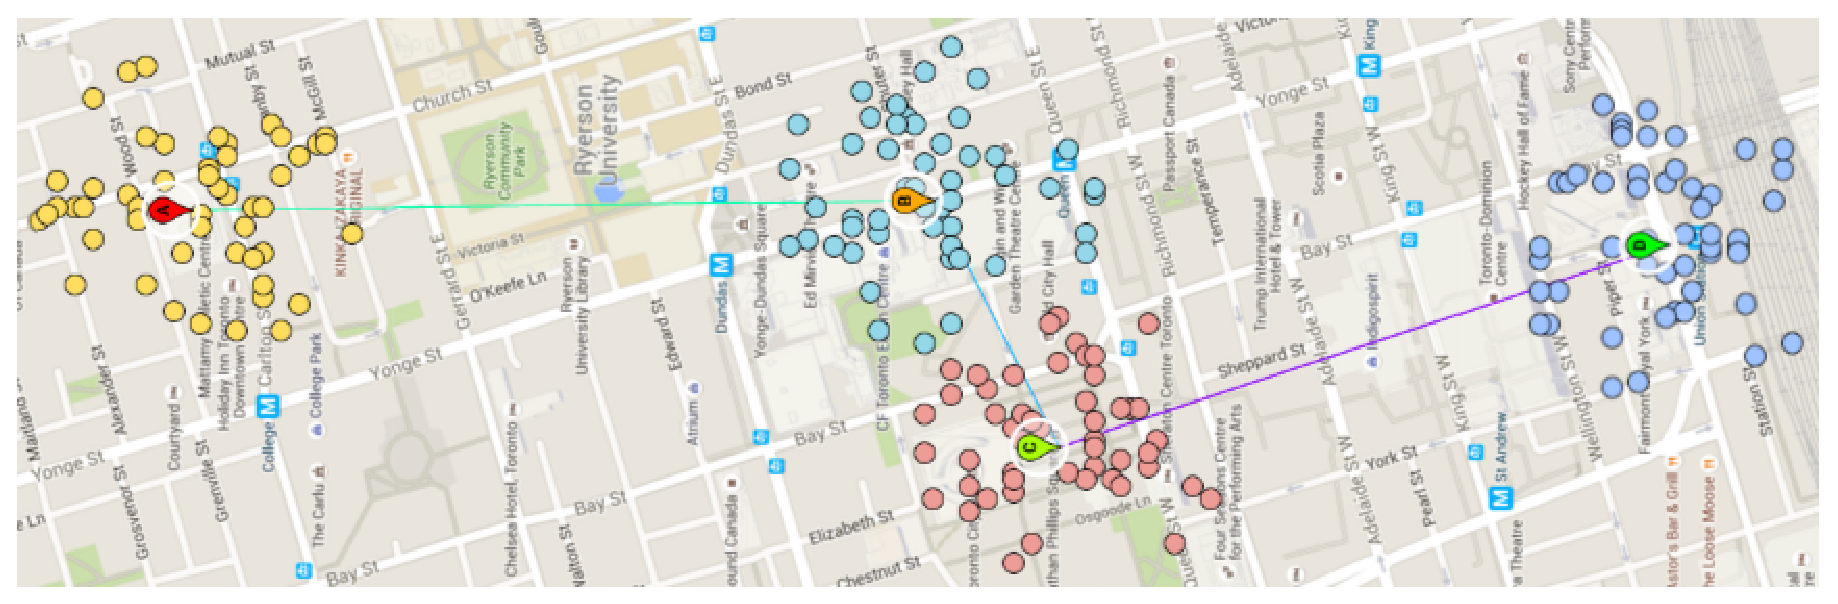
\epsfig{file=traj_eg.eps, width=3.5in}
\caption{An example of trajectory}
\label{fig:traj}
\end{figure}

\begin{table*}
\centering
\caption{Datasets description}
\label{table:data:all}
\begin{tabular}{lrrrrr} \hline
\textbf{Dataset} & \textbf{\#Photos} & \textbf{\#POI Visits} & \textbf{\#Trajectories} & \textbf{\#Users} \\ \hline
Edinburgh & 82,060 & 33,944 & 5,028 & 1,454 \\ 
Glasgow & 29,019 & 11,434 & 2,227 & 601 \\ 
Osaka & 392,420 & 7,747 & 1,115 & 450 \\ 
Toronto & 157,505 & 39,419 & 6,057 & 1,395 \\ 
\hline
\end{tabular}
\end{table*}


\subsection{Evaluation Metrics}
\label{experiment:metric}
We use leave-one-out cross validation to evaluate different trajectory recommendation algorithms,
i.e., when evaluating a specific trajectory of a user, all other trajectories of this user as well as 
all trajectories of other users are used to train the recommendation algorithm.

To evaluate the performance of different trajectory recommendation algorithms,
we employ the trajectory F$_1$-score define in \cite{ijcai15} to measure the POIs that are 
correctly recommended. Let $\mathcal{T}_a$ be the trajectory that was visited in the real world,
and $\mathcal{T}_r$ be the trajectory recommended by one of the algorithms,
trajectory F$_1$-scores was defined as
\begin{displaymath}
    F_1 = \frac{2 |\mathcal{T}_a \cap \mathcal{T}_r|}{|\mathcal{T}_a| + |\mathcal{T}_r|}
\end{displaymath}

In addition, we adapted Kendall's $\tau$ coefficient \cite{kendalltau} to measure the quality of 
recommended visiting order of POIs, which was defined as
\begin{displaymath}
    \tau = \frac{2(N_c - N_d)}{N(N-1)}
\end{displaymath}
where $N_c$ is the number of concordant pairs of POIs in the real visited trajectory $\mathcal{T}_a$ and 
the recommended trajectory $\mathcal{T}_r$, $N_d$ is the number of discordant pairs of POIs in 
$\mathcal{T}_a$ and $\mathcal{T}_r$, $N = |\mathcal{T}_a|$ is the number of visited POIs.


\subsection{Comparison}
% the way to binning POI features, #clusters of POIs,
\label{experiment:comparison}

We compared the experimental results on trajectory datasets between the proposed methods and other 7 methods:
\begin{itemize}
\item Random: choose POIs uniformly at random (without replacement) from the set of POIs $\mathcal{P} \setminus \{p_s, p_e \}$ to visit.
\item PersTour-T.5\cite{ijcai15}: personalised trajectory recommendation method described in \cite{ijcai15}, 
      time-based user interest was used and $\eta = 0.5$.
\item PersTour-T1\cite{ijcai15}: the same as PersTour-T.5, but set $\eta=1.0$.
\item PersTour-L.5: PersTour\cite{ijcai15} with budget constraint replaced with the number POIs to visit, i.e., $L$,
      similar to PersTour, we use time-based user interest and set $\eta$ to $0.5$.
\item PersTour-L1: the same as PersTour-L.5, but set $\eta=1.0$.
\item RankP: choose POIs according to the ranking based on POI popularity.
\item RankF: choose POIs according to the ranking based on POI features described in section \ref{method:ranking}.
\item MC-DP: recommend trajectory according to the Markov Chain with transition matrix described in section \ref{method:transition},
      use Viterbi algorithm to compute the most likely trajectory w.r.t. constraint $(p_s, p_e, L)$.
\item MC-ILP: the same as MC-DP, but use integer linear programming to compute the most likely trajectory.
\item Hybrid-DP: one of the proposed methods, combining POI ranking based on features 
      described in section \ref{method:ranking} and the Markov Chain with transition matrix described in section \ref{method:transition},
      use dynamic programming to compute the most likely trajectory w.r.t. constraint $(p_s, p_e, L)$.
\item Hybrid-ILP: the second proposed method, same as Hybrid-DP,
      but use integer linear programming to compute the most likely trajectory.
\item SSVM: structured prediction using EdgeFeatureGraphCRF with OneSlackSSVM to recommend trajectory.
\end{itemize}

The F$_1$-scores of different algorithms on five datasets are shown in table \ref{table:f1}
and the values of $\tau$ of different algorithms are show in table \ref{table:tau}
\footnote{We can not compute $\tau$ for PersTour-T.5 because the number of POIs in recommend trajectory is not guaranteed to equal the number of POIs in real trajectory}.

\subsection{Parameters}
For all algorithms that utilizing ranking probabilities of POIs, namely, RankF, Hybrid-DP and Hybrid-ILP,
the regularization parameter of rankSVM was $10$.
The discretization parameters used to factorize the transition probabilities between POIs was $5$, namely,
either discretizing POI features into $5$ bins in log-space or clustering POIs to $5$ clusters according to the geographical coordinates.
The trade-off parameters $\alpha$ and $\beta$ was set to $0.5$ in both Hybrid-DP and Hybrid-ILP algorithms.
The regularization parameter when training Structured SVM was $1$.


%\begin{tabular}{c|ccccccc|cccccccc} \hline
%\multirow{2}{*}{Dataset} & \multicolumn{7}{|c|}{User agnostic} & \multicolumn{8}{|c}{User specific} \\ \cline{2-15}
%                         & Rand & RankP & RankF & MC-DP & MC-ILP & Pro-DP & Pro-ILP 
%                         & PersTour & PersTour-L & RankP & RankF & MC-DP & MC-ILP & Pro-DP & Pro-ILP \\ \hline
%Toronto           & $1\pm0$ & $1\pm0$ & $1\pm0$ & $1\pm0$ & $1\pm0$ & $1\pm0$ & $1\pm0$ 
%                  & $1\pm0$ & $1\pm0$ & $1\pm0$ & $1\pm0$ & $1\pm0$ & $1\pm0$ & $\mathbf{1\pm0}$ & $1\pm0$ \\


\begin{table*}
\centering
\caption{Performance comparison on four datasets in terms of trajectory F$_1$-score}
\label{table:f1}
\begin{tabular}{l|cccc} \hline
 & Edinburgh & Glasgow & Osaka & Toronto \\ \hline
Random & $0.577\pm0.126$ & $0.632\pm0.124$ & $0.621\pm0.117$ & $0.621\pm0.128$ \\
PersTour-T.5 & $0.649\pm0.250$ & $\mathbf{0.802\pm0.213}$ & $0.702\pm0.230$ & $0.720\pm0.215$ \\
PersTour-T1 & $0.585\pm0.218$ & $0.720\pm0.211$ & $0.640\pm0.195$ & $0.710\pm0.219$ \\
PersTour-L.5 & $0.632\pm0.095$ & $0.660\pm0.102$ & $0.691\pm0.138$ & $0.642\pm0.112$ \\
PersTour-L1 & $0.599\pm0.132$ & $0.641\pm0.114$ & $0.657\pm0.141$ & $0.612\pm0.114$ \\
RankP & $0.706\pm0.159$ & $0.745\pm0.166$ & $0.661\pm0.128$ & $0.679\pm0.120$ \\
RankF & $0.707\pm0.176$ & $0.777\pm0.169$ & $0.678\pm0.116$ & $\mathbf{0.753\pm0.167}$ \\
MC-DP & $0.675\pm0.192$ & $0.717\pm0.170$ & $0.679\pm0.162$ & $0.662\pm0.156$ \\
MC-ILP & $0.707\pm0.159$ & $0.735\pm0.170$ & $0.706\pm0.154$ & $0.688\pm0.139$ \\
Hybrid-DP & $0.692\pm0.198$ & $0.739\pm0.178$ & $0.705\pm0.171$ & $0.691\pm0.171$ \\
Hybrid-ILP & $\mathbf{0.727\pm0.163}$ & $0.763\pm0.171$ & $\mathbf{0.718\pm0.163}$ & $0.726\pm0.152$ \\
SSVM & - & $0.727\pm0.173$ & $0.715\pm0.170$ & $0.728\pm0.186$ \\
\hline
\end{tabular}
\end{table*}


\begin{table*}
\centering
\caption{Performance comparison on four datasets in terms of $\tau$}
\label{table:tau}
\begin{tabular}{l|cccc} \hline
 & Edinburgh & Glasgow & Osaka & Toronto \\ \hline
Random & $0.261\pm0.119$ & $0.318\pm0.165$ & $0.305\pm0.145$ & $0.309\pm0.166$ \\
PersTour-L.5 & $0.311\pm0.109$ & $0.349\pm0.163$ & $0.415\pm0.243$ & $0.329\pm0.158$ \\
PersTour-L1 & $0.287\pm0.168$ & $0.331\pm0.159$ & $0.361\pm0.218$ & $0.292\pm0.134$ \\
RankP & $0.440\pm0.258$ & $0.503\pm0.296$ & $0.361\pm0.194$ & $0.378\pm0.203$ \\
RankF & $0.438\pm0.287$ & $\mathbf{0.557\pm0.306}$ & $0.373\pm0.186$ & $0.508\pm0.297$ \\
MC-DP & $0.481\pm0.269$ & $0.478\pm0.286$ & $0.442\pm0.259$ & $0.404\pm0.229$ \\
MC-ILP & $0.442\pm0.278$ & $0.485\pm0.295$ & $0.445\pm0.268$ & $0.399\pm0.233$ \\
Hybrid-DP & $0.500\pm0.288$ & $0.531\pm0.299$ & $0.495\pm0.276$ & $0.451\pm0.264$ \\
Hybrid-ILP & $0.484\pm0.283$ & $0.531\pm0.309$ & $0.470\pm0.288$ & $0.459\pm0.269$ \\
SSVM & - & $0.505\pm0.282$ & $\mathbf{0.499\pm0.293}$ & $\mathbf{0.511\pm0.312}$ \\
\hline
\end{tabular}
\end{table*}

\subsection{Avoid Peeking}
When working with machine learning methods, to make sure the reported performance is a good approximation
of the generalization performance, it is critical to prevent information in test set from leaking into
training set.
Many algorithms in the above comparison utilizing both learning to rank and factorized Markov Chain, 
e.g., Hybrid-DP, Hybrid-ILP and SSVM,
both of them need to be trained or parameters be estimated before being used in other algorithms.
Features such as popularity of a POI, the number of visits of a POI and the average visit duration at a POI are
determined by the POI itself as well as trajectories in training set, let's call them aggregated features as they are 
computed by aggregating a set of trajectories.
To make the prediction performance is reliable, it is very important to not include trajectories in test set 
when computing aggregated features.
Unfortunately, it is quite easy, especially when utilizing multiple levels of machine learning models,
to use all data, including those in test set, to compute aggregated features and many researchers and 
practitioners did not realize some bits of information in test set were leaked into training set via these aggregated features.

%One may argue that many of these features will not change much when computed with or without data in test set,
%but in certain areas, such as aerodynamics, some decisions are very sensitive to the quantity of certain features.
%Nevertheless, the exact impact still needs further investigation.

\subsection{Analysis of Experimental Results}

\label{experiment:analysis}
